\documentclass[a4paper]{scrartcl}
\usepackage{makecell}
\usepackage{multicol}
\usepackage{graphicx}
\usepackage{anysize}
\usepackage{amsmath}
\usepackage{kpfonts}
\usepackage{tabularx}
\usepackage{hyperref}
\usepackage{listings}
\usepackage{color}
\usepackage[parfill]{parskip}

\marginsize{25mm}{25mm}{25mm}{25mm}
%---Code-Editor Config ------------------------%
\definecolor{dkgreen}{rgb}{0,0.6,0}
\definecolor{gray}{rgb}{0.5,0.5,0.5}
\definecolor{mauve}{rgb}{0.58,0,0.82}
\definecolor{backcolour}{rgb}{0.95,0.95,0.92}
\lstset{basicstyle=\ttfamily}
\lstset{literate=%
    {á}{{\'a}}1 {é}{{\'e}}1 {í}{{\'i}}1 {ó}{{\'o}}1 {ú}{{\'u}}1
    {Á}{{\'A}}1 {É}{{\'E}}1 {Í}{{\'I}}1 {Ó}{{\'O}}1 {Ú}{{\'U}}1
	{à}{{\`a}}1 {è}{{\`e}}1 {ì}{{\`i}}1 {ò}{{\`o}}1 {ù}{{\`u}}1
	{À}{{\`A}}1 {È}{{\'E}}1 {Ì}{{\`I}}1 {Ò}{{\`O}}1 {Ù}{{\`U}}1
	{ä}{{\"a}}1 {ë}{{\"e}}1 {ï}{{\"i}}1 {ö}{{\"o}}1 {ü}{{\"u}}1
	{Ä}{{\"A}}1 {Ë}{{\"E}}1 {Ï}{{\"I}}1 {Ö}{{\"O}}1 {Ü}{{\"U}}1
	{â}{{\^a}}1 {ê}{{\^e}}1 {î}{{\^i}}1 {ô}{{\^o}}1 {û}{{\^u}}1
	{Â}{{\^A}}1 {Ê}{{\^E}}1 {Î}{{\^I}}1 {Ô}{{\^O}}1 {Û}{{\^U}}1
	{œ}{{\oe}}1 {Œ}{{\OE}}1 {æ}{{\ae}}1 {Æ}{{\AE}}1 {ß}{{\ss}}1
	{ç}{{\c c}}1 {Ç}{{\c C}}1 {ø}{{\o}}1 {å}{{\r a}}1 {Å}{{\r A}}1
	{€}{{\EUR}}1 {£}{{\pounds}}1
	{>}{{$>$}}1{<}{{$<$}}1
}
\lstset{
	language=Python,				% the language of the code
	basicstyle=\footnotesize,			% the size of the fonts that are used for the code
	numbers=left,					% where to put the line-numbers
	numberstyle=\tiny\color{gray},		% the style that is used for the line-numbers
	stepnumber=1,					% the step between two line-numbers. If it's 1, each line will be numbered
	numbersep=5pt,				% how far the line-numbers are from the code
	backgroundcolor=\color{white},		% choose the background color. You must add \usepackage{color}
	showspaces=false,				% show spaces adding particular underscores
	showstringspaces=false,			% underline spaces within strings
	showtabs=false,				% show tabs within strings adding particular underscores
	frame=single,					% adds a frame around the code
	rulecolor=\color{black},			% if not set, the frame-color may be changed on line-breaks within not-black text (e.g. commens (green here))
	tabsize=2,						% sets default tabsize to 2 spaces
	captionpos=b,					% sets the caption-position to bottom
	breaklines=true,                			% sets automatic line breaking
  	breakatwhitespace=false,       		% sets if automatic breaks should only happen at whitespace
  	title=\lstname,        % show the filename of files included with \lstinputlisting; % also try caption instead of title
  	keywordstyle=\color{blue},          	% keyword style
  	commentstyle=\color{dkgreen},       	% comment style
  	stringstyle=\color{mauve},         		% string literal style
  	escapeinside={\%*}{*)},            		% if you want to add LaTeX within your code
  	morekeywords={*,...}              		% if you want to add more keywords to the set
}

%Header and Footer -----------------------%
\usepackage[headsepline]{scrlayer-scrpage}
\pagestyle{scrheadings}
\clearpairofpagestyles
%\setlength{\headheight}{40.8pt}
\setlength{\headheight}{56pt}
\ihead{IRTM\\ Wi 20/21\\ Assigment 4} 
\ohead{
    Alberto Saponaro - saponaroalberto97@gmail.com\\
    Walter Väth - walter.vaeth@gmail.com\\
    Chong Shen - st143575@stud.uni-stuttgart.de\\
    Xin Pang - st145113@stud.uni-stuttgart.de
}
\ofoot{\pagemark}



%-----------------------------------------------%
%  BEGIN                                        %
%-----------------------------------------------%
\begin{document}
    
\section*{Task 1}
\textbf{Vocabulary} = \{ happy, new, year, holiday, term, starts, work, celebrations \}\\
$|$Vocabulary$|$ = 8

\subsubsection*{Prior:}
    $P(c_1) = \frac{3}{5} = 0.6$\\
    $P(c_2) = \frac{2}{5} = 0.4$ 

\subsubsection*{Posterior: (with Add-One-Smoothing)}
\begin{multicols}{2}
    $P(happy|c_1) = \frac{2 + 1}{7 + 8} = \frac{3}{15}$\\
    $P(new|c_1) = \frac{2 + 1}{7 + 8} = \frac{3}{15}$\\
    $P(year|c_1) = \frac{2 + 1}{7 + 8} = \frac{3}{15}$\\
    $P(holiday|c_1) = \frac{1 + 1}{7 + 8} = \frac{2}{15}$\\
    $P(term|c_1) = \frac{0 + 1}{7 + 8} = \frac{1}{15}$\\
    $P(starts|c_1) = \frac{0 + 1}{7 + 8} = \frac{1}{15}$\\
    $P(work|c_1) = \frac{0 + 1}{7 + 8} = \frac{1}{15}$\\
    $P(celebrations|c_1) = \frac{0 + 1}{7 + 8} = \frac{1}{15}$

    $P(happy|c_2) = \frac{0 + 1}{4 + 8} = \frac{1}{12}$\\
    $P(new|c_2) = \frac{0 + 1}{4 + 8} = \frac{1}{12}$\\
    $P(year|c_2) = \frac{0 + 1}{4 + 8} = \frac{1}{12}$\\
    $P(holiday|c_2) = \frac{0 + 1}{4 + 8} = \frac{1}{12}$\\
    $P(term|c_2) = \frac{1 + 1}{4 + 8} = \frac{2}{12}$\\
    $P(starts|c_2) = \frac{2 + 1} + 1{4 + 8} = \frac{3}{12}$\\
    $P(work|c_2) = \frac{1 + 1}{4 + 8} = \frac{2}{12}$\\
    $P(celebrations|c_2) = \frac{0 + 1}{4 + 8} = \frac{1}{12}$
\end{multicols}

$P(c_1|d) = \frac{3}{5} * \frac{3}{15} * \frac{3}{15} * \frac{3}{15} * \frac{1}{15} = \frac{81}{253125} = c_{map}$\\
$P(c_2|d) = \frac{1}{12} * \frac{1}{12} * \frac{1}{12} * \frac{1}{12} = \frac{2}{103680}$

The model assigned the class $c_1$ to the document.

\section*{Task 2}
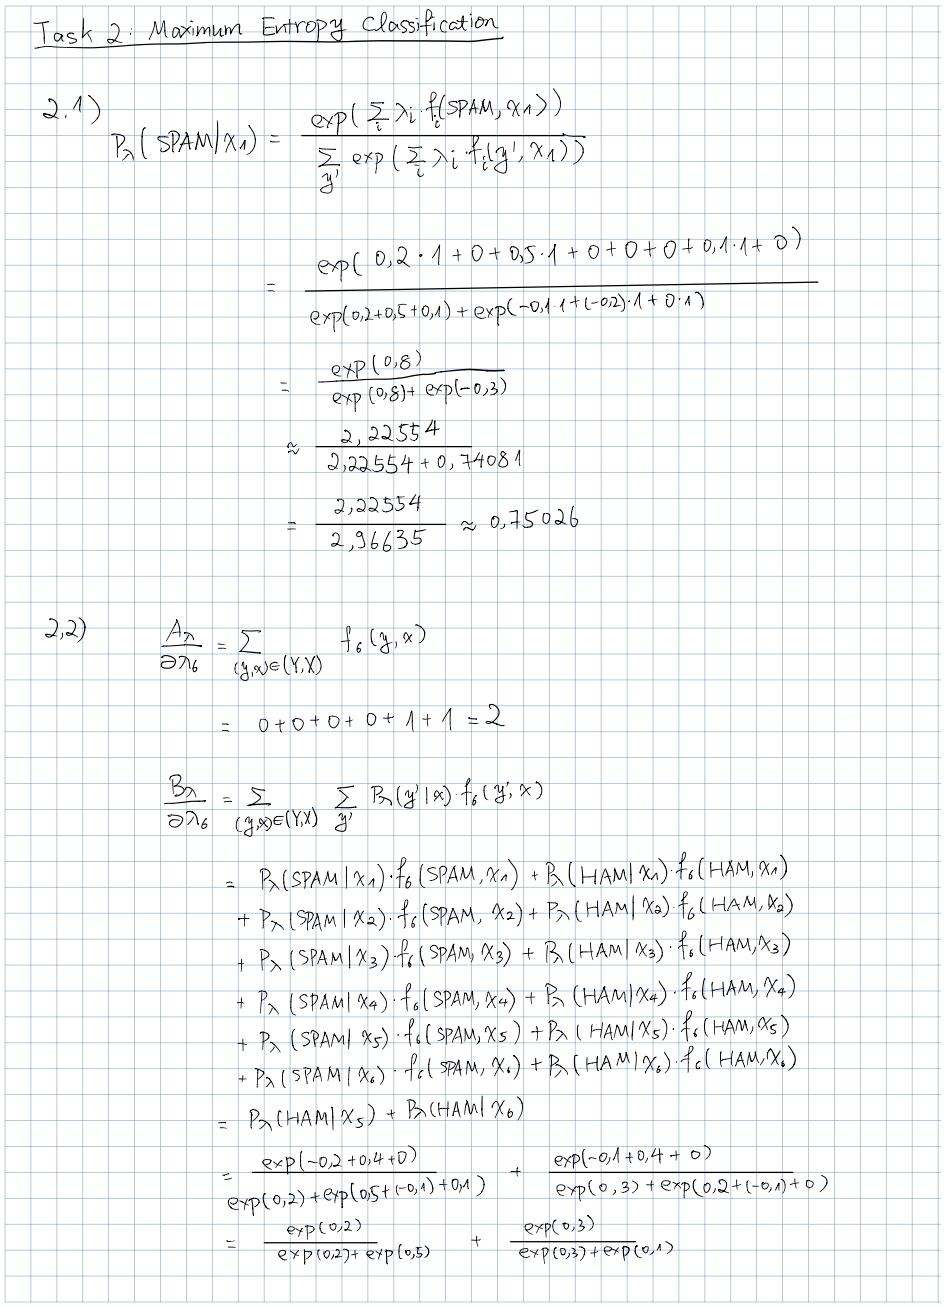
\includegraphics[width=.9\textwidth]{img/task2a.png}
\newpage
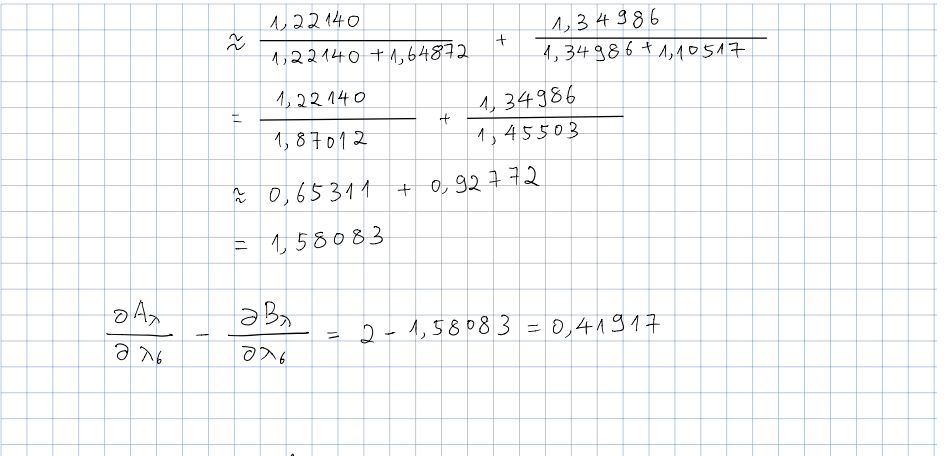
\includegraphics[width=.9\textwidth]{img/task2b.png}


\pagebreak
\section*{Task 3}
\begin{itemize}
	\item k=1\\ $P(black|x)=0$\\ $P(white|x)=\frac{1}{1} = 1$
	\item k=3\\ $P(black|x)=\frac{1}{3}$\\ $P(white|x)=\frac{2}{3}$
	\item k=5\\ $P(black|x)=\frac{2}{5}$\\ $P(white|x)=\frac{3}{5} = 1$
\end{itemize}
$\frac{3}{5}<\frac{2}{3}<1$\\ 
In case of k=5 the kNN classifier hast the lowest classification confidence.







\section*{Programming Task}
\lstinputlisting{code/script.py}
\subsubsection*{OUTPUT:}
\begin{lstlisting}
	-------------------------------------------------- 
	Top 100 result for class 'gut': 
	--------------------------------------------------
	 24534          spiel
	 22102          !
	 19037          ist
	 18307          es
	 15812          cool
	 14978          das
	 13549          .
	 12106          macht
	 10989          :
	 10854          super
	 10760          ich
	 10104          und
	 10019          )
	 9793   geil
	 8686   aber
	 8514   gut
	 8346   sehr
	 7933   einfach
	 7425   man
	 7323   spaß
	 7083   ,
	 6499   ein
	 6411   nur
	 6316   die
	 4627   echt
	 4427   -
	 4038   finde
	 3973   so
	 3931   zu
	 3847   noch
	 3601   viel
	 3489   nachbarn
	 3476   auch
	 3024   süchtig
	 2906   kann
	 2805   suche
	 2802   für
	 2692   richtig
	 2586   der
	 2569   mich
	 2531   toll
	 2478   wenn
	 2464   ;
	 2463   game
	 2439   mit
	 2390   gutes
	 2365   dieses
	 2252   voll
	 2128   adden
	 2127   spiele
	 2058   liebe
	 2051   cooles
	 2023   top
	 1967   hammer
	 1934   tolles
	 1900   bin
	 1765   *
	 1717   mir
	 1686   neue
	 1679   hat
	 1668   geiles
	 1647   beste
	 1637   sind
	 1623   sonst
	 1616   immer
	 1602   ...
	 1541   weiter
	 1531   klasse
	 1471   muss
	 1451   alles
	 1431   langweilig
	 1428   bitte
	 1420   freunde
	 1411   manchmal
	 1394   wie
	 1385   zeitvertreib
	 1350   app
	 1337   also
	 1329   spass
	 1298   ganz
	 1271   gibt
	 1250   lol
	 1240   is
	 1227   5
	 1202   sterne
	 1198   mega
	 1189   wäre
	 1176   was
	 1153   eine
	 1131   auf
	 1114   spielen
	 1087   läuft
	 1062   könnte
	 1057   empfehlen
	 1057   dass
	 1040   ihr
	 1000   wirklich
	 991    weil
	 987    jeden
	 985    nie
   
   
   
   
   -------------------------------------------------- 
	Top 100 result for class 'schlecht': 
	--------------------------------------------------
	 -2016          nicht
	 -1837          mehr
	 -1183          seit
	 -987   update
	 -953   beheben
	 -902   komme
	 -721   rein
	 -711   ?
	 -711   ins
	 -678   weg
	 -641   event
	 -632   war
	 -619   stürzt
	 -588   geht
	 -564   dem
	 -542   nichts
	 -534   ständig
	 -498   soll
	 -473   keinen
	 -453   heute
	 -419   letzten
	 -408   verbindung
	 -407   gar
	 -367   neu
	 -359   komm
	 -355   ab
	 -353   server
	 -350   deinstalliert
	 -343   anfangen
	 -321   tagen
	 -318   fehler
	 -308   starten
	 -303   vorne
	 -303   scheiße
	 -302   scheiß
	 -299   nix
	 -279   gelöscht
	 -269   startet
	 -257   behebt
	 -255   lässt
	 -246   werde
	 -226   öffnen
	 -221   22
	 -218   wieder
	 -218   steht
	 -217   stern
	 -210   möglich
	 -208   obwohl
	 -202   nun
	 -198   mist
	 -191   dann
	 -190   support
	 -189   0
	 -176   gestern
	 -170   spielstand
	 -168   null
	 -165   %
	 -157   schlüssel
	 -154   lädt
	 -150   kotzen
	 -145   -.-
	 -143   wurde
	 -137   1
	 -137   gekauft
	 -136   anmelden
	 -136   zynga
	 -134   behoben
	 -133   enttäuscht
	 -132   sauer
	 -130   bekomme
	 -129   wollte
	 -127   raus
	 -125   investiert
	 -121   zurück
	 -121   passiert
	 -119   bildschirm
	 -118   beendet
	 -115   sofort
	 -115   deinstallieren
	 -114   abzocke
	 -113   belohnung
	 -113   scheisse
	 -112   installiert
	 -112   dauernd
	 -111   beim
	 -108   laden
	 -106   langsam
	 -106   installieren
	 -105   ärgerlich
	 -104   andauernd
	 -103   wochen
	 -99    seid
	 -98    trotz
	 -97    sekunden
	 -96    morgen
	 -95    zeigt
	 -94    angezeigt
	 -93    plötzlich
	 -91    bricht
	 -89    müll	
\end{lstlisting}


\end{document}